\documentclass{beamer}
\usepackage[utf8]{inputenc}


\usepackage{amsmath}
\usepackage{amssymb}
\usepackage{amsthm}
\usepackage{amsfonts}
% \usepackage{xcolor}
\usepackage{graphicx}

\usepackage{tikz}


\usepackage[space]{grffile}


% --- Partie code
\usepackage{listings}
\lstset{language=C,
        showstringspaces=false,
        basicstyle=\footnotesize\ttfamily,
        captionpos=b,
        stepnumber=1,
        keywordstyle=\bfseries\color{green!40!black},
        commentstyle=\itshape\color{purple!40!black},
        identifierstyle=\color{blue},
        stringstyle=\color{red}}

\newcommand{\cl}[1]{\texttt{#1}}

\newcommand{\mut}{\textbf{mutable }}
\newcommand{\nmut}{\textbf{non-mutable }}
\newcommand{\bang}{\textbf{mutable }}
\newcommand{\safe}{\textbf{safe }}
\newcommand{\dupl}{\textbf{duplicated }}


% --- Parti math. (app.)
%\newtheorem{theorem}{Theorem}
%\newtheorem{lemma}[theorem]{Lemma}
%\newtheorem{proposition}[theorem]{Proposition}
%\newtheorem{corollary}[theorem]{Corollary}
%\newtheorem{definition}[theorem]{Definition}
%\newtheorem{algorithm}[theorem]{Algorithm}
%\newtheorem{remark}[theorem]{Remark}

% Mathematic abbreviations
\newcommand{\N}{\mathbb{N}}
\newcommand{\Z}{\mathbb{Z}}
\newcommand{\Q}{\mathbb{Q}}
\newcommand{\R}{\mathbb{R}}

\newcommand{\mpzt}{ \texttt{ mpz\_t } }
\newcommand{\mpqt}{ \texttt{ mpq\_t } }

% evaluation context hole
\newcommand{\econt}[1]{[#1]}
% update context hole
\newcommand{\ucont}[1]{\{#1\}}



\usetheme{Boadilla}
\usecolortheme{beaver}


\title[From PVS to C]{Translating PVS to C}
\subtitle{SRI International}
\author[Gaspard Férey]{Gaspard Férey}
\institute{Ecole Polytechnique}
\date{September 1st, 2014}


\begin{document}

\frame{\titlepage}

\begin{frame}
\frametitle{Table of Contents}
\tableofcontents
% \tableofcontents[currentsection]
\end{frame}


\section{Context}

\begin{frame}
\frametitle{Table of Contents}
\tableofcontents[currentsection]
\end{frame}


\begin{frame}
\frametitle{What is PVS ?}

\begin{itemize}
\itemsep2em
\item A specification language
\begin{itemize}
\item Typed expression definition
\item Theories, datatypes, ...
\end{itemize}
\item A semi automated theorem prover
\begin{itemize}
\item Higher order logic
\item Type system, judgments, ...
\item Theorems, properties, ...
\item SMT solvers integrated, tools, ...
\end{itemize}
\item A functional programming language (?)
\end{itemize}

\end{frame}


\begin{frame}
\frametitle{Why translate PVS ?}

\begin{itemize}
\itemsep2em
\item To be able to execute PVS
\begin{itemize}
\item Testing
\item Debugging
\end{itemize}
\item To integrate high-insurance PVS code into systems
\end{itemize}

\end{frame}





\section{Static analysis}
\begin{frame}
\frametitle{Table of Contents}
\tableofcontents[currentsection]
\end{frame}

\subsection{The update issue}

\begin{frame}
\frametitle{Update expression}
\begin{itemize}
\itemsep2em
\item In functional programming languages,
$$ E := A \cl{ WITH [($x$) := $y$]} $$
refers $i \mapsto \left\lbrace \begin{array}{ll}
A(i) & \text{if $i \neq x$} \\
y & \text{if } i = x
\end{array} \right. $
\item In imperative languages
\begin{itemize}
\item \cl{A[x := y]} a non destructive update using a copy of $A$.
\item \cl{A[x <- y]} a destructive, in-place update of the aggregate structure representing A.
\end{itemize}
\end{itemize}

\end{frame}


\begin{frame}
\frametitle{Two dangers}
\begin{itemize}
\itemsep2em
\item Unsafe occurrence
$$ \cl{LET B = A WITH[(0) := 0] IN B(0) + A(0)} $$
The array represented by \cl{A} is used later in the code.
\item Trapped reference
$$ \cl{LET A = B(0) IN f( A WITH [(0) := 0], B(0) )} $$
\cl{B} is affected by a destructive update of the array represented by \cl{A}.
\end{itemize}

\end{frame}


\begin{frame}
\frametitle{Previous analysis}
Shankar's analysis relies on sets of \emph{variables}
\begin{itemize}
\item $Av$ active variables
\item $Ov$ output variables
\item $Fv$ free variables
\item $Lv$ live variables in an \emph{update context}
\end{itemize}
\ \newline
Cerny and Shankar's analysis adds \emph{flow analysis}.
\end{frame}



\subsection{Reference tracking}

\begin{frame}
\frametitle{The intermediate language}
\begin{columns}
\begin{column}{0.45\textwidth}
Syntax
\begin{itemize}
\item Integers, nil pointer
\item Variables (\cl{X}, \cl{x}, \cl{y}, ...)
\item \cl{newArray(x, y)}
\item \cl{X[x := y]}
\item \cl{X[x <- y]}
\item \cl{X[x]}
\item \cl{let x = $a$ in $e$}
\item \cl{if(x) $e_1$ else $e_2$}
\item \cl{f($\cl{x}_1$, ... ,$\cl{x}_n$)}
\end{itemize}
\end{column}

\begin{column}{0.55\textwidth}
Memory state representation:
\begin{itemize}
\item Variables space $Var$
\item Reference space $\mathcal{R}$
\item Value space $\mathcal{V} := \N \cup \mathcal{R}$
\item Store $R : \mathcal{R} \longrightarrow \mathcal{V}$
\item Stack $S : Var \longrightarrow \mathcal{V}$
\end{itemize}
\ \newline
Evaluation context
\begin{itemize}
\item hole $\{\}$
\item \cl{let x = $\{\}$ in $e$}
\item $E_1\{E_2\}$
\end{itemize}
\end{column}
\end{columns}

\end{frame}

\begin{frame}
\frametitle{The intermediate language}
\framesubtitle{Operational semantics}
Simple reduction rules:
\begin{eqnarray*}
<x | R, S> &\rightarrow& < S(x)|R,S> \\
<x \cl{[} y \cl{]} | R, S> &\rightarrow & < R(S(x))(S(y))|R,S> \\
<\cl{if(x) } a \cl{ else } b |R,S> &\rightarrow&
\left\lbrace \begin{array}{ll}
<b|R,S> & \text{if } S(x) = 0 \\
<a|R,S> & \text{otherwise}
\end{array} \right.
\end{eqnarray*}
Introducing variables
\begin{eqnarray*}
<f\cl{(} x_1, ... , x_n \cl{)} | R, S> &\rightarrow& < \cl{pop(} [f] \cl{)} | R, \left( \biguplus_{1 \leq i \leq n} f_i \mapsto S(x_i) \right) :: S > \\
<\cl{let } x \cl{ = } v \cl{ in } e | R, S> &\rightarrow& < \cl{pop(}e\cl{)}|R, (x \mapsto v) :: S > \\
<\cl{pop(} v \cl{)} | R, S> &\rightarrow& <v | R, pop(S) >
\end{eqnarray*}
\end{frame}



\begin{frame}
\frametitle{The intermediate language}
\framesubtitle{Operational semantics}
Modifying the store
\begin{eqnarray*}
<\cl{newArray(} x, y \cl{)} | R, S> &\rightarrow& <r| R\uplus \left( r \mapsto (S(y))_{0 \leq i < S(x)} \right), S> \\
&\text{where}& r \text{ is a fresh pointer} \\
< X \cl{[} x \cl{ := } y \cl{]} | R, S> &\rightarrow& < r| R', S> \\
&\text{where}& r \text{ fresh pointer} \\
&\text{and}& R' := R \uplus \left( r \mapsto A \right) \\
&\text{and}& A  := R( S(X) ) \uplus \left( S(x) \mapsto S(y) \right) \\
< X \cl{[} x \cl{ <- } y \cl{]} | R, S> &\rightarrow& < X| R', S> \\
&\text{where}& R' := R \uplus \left( S(X) \mapsto A \right) \\
&\text{and}&   A  := R( S(X) ) \uplus \left( s(x) \mapsto S(y) \right)
\end{eqnarray*}
\end{frame}


\begin{frame}[fragile]
\frametitle{Reference graph}
For a context in the body of a function
\begin{lstlisting}
f(A, B) =
  let C = if(A[0] = 1) then A else B in
  let D =
    let E = C in E[0 := 0] in
  D[0] + A(0)
\end{lstlisting}
we can define the reference graph $\mathcal{G}(R)(r)$ as
\begin{eqnarray*}
r &\in& \mathcal{G}(r) \\
\mathcal{R} \cap R(\mathcal{G}(r)) &\subset& \mathcal{G}(r)
\end{eqnarray*}
We are interested in
$$ \bigcup_{R} \ S^{-1}( \ \mathcal{G}(R)(S(x)) \ )  $$
\end{frame}


\begin{frame}[fragile]
\frametitle{Reference graph}
\begin{columns}
\begin{column}{0.5\textwidth}
Definition of \cl{f}
\begin{lstlisting}
f(A, B) =
  let C = A[0]      in
  let D = C[0 := 0] in
  let E = g(B)      in
  let X = E[0 := 0] in
  let F = if X[0] then D
                  else X in
  let G = F[0 := 0] in
  let H = if B[0] then G
                  else B in
  H[0 := B[0]]
\end{lstlisting}
\end{column}
\begin{column}{0.5\textwidth}
\end{column}
\end{columns}
\end{frame}



\begin{frame}[fragile]
\frametitle{Reference graph}
\begin{columns}
\begin{column}{0.5\textwidth}
\begin{lstlisting}
f(A, B) =
  let C = A[0]      in
  let D = { C }     in
  let E = g(B)      in
  let X = E[0 := 0] in
  let F = if X[0] then D
                  else X in
  let G = F[0 := 0] in
  let H = if B[0] then G
                  else B in
  H[0 := B[0]]
\end{lstlisting}
\end{column}
\begin{column}{0.5\textwidth}
Reference graph
\begin{center}
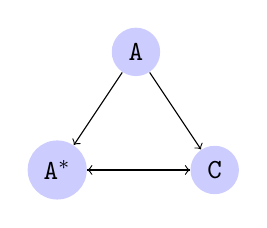
\begin{tikzpicture}
  [scale=.5,every node/.style={circle,fill=blue!20}]
  \node (n1) at (3,4) {\cl{A}};
  \node (n2) at (1,1)  {$\cl{A}^*$};
  \node (n3) at (5,1)  {\cl{C}};

  \foreach \from/\to in {n1/n2,n1/n3,n2/n3,n3/n2}
    \draw[->] (\from) -- (\to);
\end{tikzpicture}
\end{center}
\ \newline
Variables lives in the context
$$\{ \cl{B}, \cl{D}, \cl{E}, \cl{F}, \cl{G}, \cl{H}, \cl{X} \}$$
\end{column}
\end{columns}
\ \newline \ \newline
Destructive update would impose too many requirements to $f$.
\end{frame}



\begin{frame}[fragile]
\frametitle{Reference graph}
\begin{columns}
\begin{column}{0.5\textwidth}
Definition of \cl{f}
\begin{lstlisting}
f(A, B) =
  let C = A[0]      in
  let D = C[0 := 0] in
  let E = g(B)      in
  let X = { E }     in
  let F = if X[0] then D
                  else X in
  let G = F[0 := 0] in
  let H = if B[0] then G
                  else B in
  H[0 := B[0]]
\end{lstlisting}
\end{column}
\begin{column}{0.5\textwidth}
Reference graph
\begin{center}
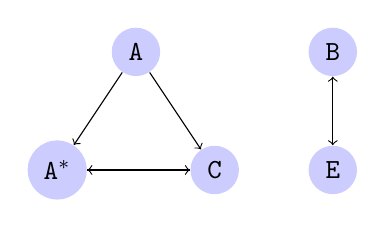
\begin{tikzpicture}
  [scale=.5,every node/.style={circle,fill=blue!20}]
  \node (n1) at (3,4) {\cl{A}};
  \node (n2) at (1,1)  {$\cl{A}^*$};
  \node (n3) at (5,1)  {\cl{C}};
  \node (n4) at (8,1) {\cl{E}};
  \node (n5) at (8,4) {\cl{B}};

  \foreach \from/\to in {n1/n2,n1/n3,n2/n3,n3/n2,n4/n5,n5/n4}
    \draw[->] (\from) -- (\to);
\end{tikzpicture}
\end{center}
\ \newline
Variables lives in the context
$$\{ \cl{B}, \cl{C}, \cl{D}, \cl{F}, \cl{G}, \cl{H}, \cl{X} \}$$
\end{column}
\end{columns}
\ \newline \ \newline
\cl{B} is live in the context.
\end{frame}


\begin{frame}[fragile]
\frametitle{Reference graph}
\begin{columns}
\begin{column}{0.5\textwidth}
\begin{lstlisting}
f(A, B) =
  let C = A[0]      in
  let D = C[0 := 0] in
  let E = g(B)      in
  let X = E[0 := 0] in
  let F = if X[0] then D
                  else X in
  let G = { F }     in
  let H = if B[0] then G
                  else B in
  H[0 := B[0]]
\end{lstlisting}
\end{column}
\begin{column}{0.5\textwidth}
Reference graph
\begin{center}
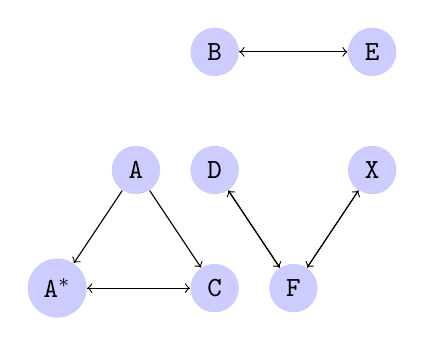
\begin{tikzpicture}
  [scale=.5,every node/.style={circle,fill=blue!20}]
  \node (n1) at (3,1) {\cl{F}};
  \node (n2) at (1,4) {\cl{D}};
  \node (n3) at (5,4) {\cl{X}};
  \node (n4) at (5,7) {\cl{E}};
  \node (n5) at (1,7) {\cl{B}};
  \node (n6) at (-1,4) {\cl{A}};
  \node (n7) at (-3,1)  {$\cl{A}^*$};
  \node (n8) at (1,1)  {\cl{C}};

  \foreach \from/\to in {n1/n2,n1/n3,n2/n1,n3/n1,n5/n4,n4/n5,n6/n7,n6/n8,n7/n8,n8/n7}
    \draw[->] (\from) -- (\to);
\end{tikzpicture}
\end{center}
Variables lives in the context
$$\{ \cl{B}, \cl{C}, \cl{G}, \cl{H} \}$$
\end{column}
\end{columns}
\ \newline \ \newline
Destructive update possible.
\end{frame}



\begin{frame}[fragile]
\frametitle{Reference graph}
\begin{columns}
\begin{column}{0.5\textwidth}
\begin{lstlisting}
f(A, B) =
  let C = A[0]      in
  let D = C[0 := 0] in
  let E = g(B)      in
  let X = E[0 := 0] in
  let F = if X[0] then D
                  else X in
  let G = F[0 <- 0] in
  let H = if B[0] then G
                  else B in
  { H }
\end{lstlisting}
\ \newline
Variables lives in the context
$$\{  \}$$
\end{column}
\begin{column}{0.5\textwidth}
Reference graph
\begin{center}
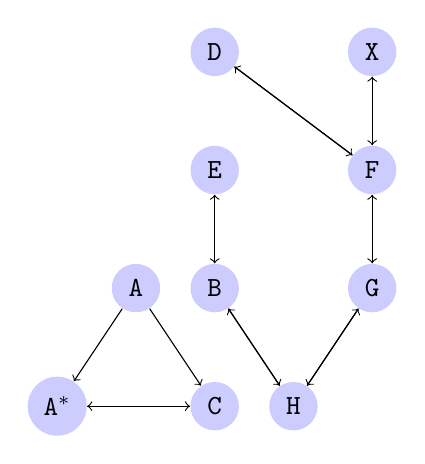
\begin{tikzpicture}
  [scale=.5,every node/.style={circle,fill=blue!20}]
  \node (n6) at (-1,4) {\cl{A}};
  \node (n7) at (-3,1) {$\cl{A}^*$};
  \node (n8) at (1,1)  {\cl{C}};
  \node (n1) at (3,1)  {\cl{H}};
  \node (n2) at (1,4)  {\cl{B}};
  \node (n3) at (5,4)  {\cl{G}};
  \node (n4) at (5,7)  {\cl{F}};
  \node (n5) at (1,7)  {\cl{E}};
  \node (n9) at (5,10) {\cl{X}};
  \node (n0) at (1,10) {\cl{D}};

  \foreach \from/\to in {n1/n2,n1/n3,n2/n1,n3/n1,n6/n7,n6/n8,n7/n8,n8/n7,n2/n5,n5/n2,n3/n4,n4/n3,n4/n9,n9/n4,n4/n0,n0/n4}
    \draw[->] (\from) -- (\to);
\end{tikzpicture}
\end{center}
\end{column}
\end{columns}
\ \newline
Destructive update possible.
\end{frame}




\subsection{Mutable analysis}

\begin{frame}
\frametitle{The flags}
We implement an approximation of the analysis using three flags
\begin{itemize}
\itemsep1.5em
\item \bang
\begin{itemize}
\item Variable: Every other variable that may point to that variable is not live.
\item Argument: Variables passed as this argument must be flagged \bang and \safe.
\item Function: The result of a call to that function is "fresh".
\end{itemize}
\item \textbf{dupl}
\begin{itemize}
\item Argument: Possible active variable in a call to this function.
\item Expression: May be aliased to the return value.
\end{itemize}
\item \textbf{safe}
\begin{itemize}
\item Last of occurrence of a variable
\end{itemize}
\end{itemize}

\end{frame}


\begin{frame}
\frametitle{The rules}
\begin{itemize}
\itemsep1em
\item Two versions for each function
\begin{itemize}
\item destructive
\item non destructive
\end{itemize}
\item \bang flag:
\begin{itemize}
\itemsep0em
\item 
\end{itemize}
\item \textbf{dupl} flag:
\begin{itemize}
\itemsep0em
\item 
\end{itemize}
\end{itemize}
\end{frame}


\begin{frame}[fragile]
\frametitle{Example}
\begin{columns}
\begin{column}{0.5\textwidth}
Destructive version of \cl{f}
\begin{lstlisting}
f(A, B) =
  let C = A[0]      in
  let D = C[0 := 0] in
  let E = g(B)      in
  let X = E[0 := 0] in
  let F = if X[0] then D
                  else X in
  let G = F[0 <- 0] in
  let H = if B[0] then G
                  else B in
  H[0 <- 0]
\end{lstlisting}
\end{column}
\begin{column}{0.5\textwidth}
\pause
\cl{C} no flags \\
\pause
\cl{D} \bang \\
$\Longleftarrow$ non destructive update\\
\pause
\cl{E} no flags \\
\pause
\cl{X} \bang \\
$\Longleftarrow$ non destructive update\\
\pause
\cl{F} \bang \\
$\Longleftarrow$ \cl{D} and \cl{X} \safe and \bang \\
\pause
\cl{G} \bang \\
$\Longleftarrow$ \cl{F} \safe and \bang \\
\pause
\cl{H} \textbf{ mutable } \\
$\Longleftarrow$ \cl{G} and \cl{B} \safe and \bang \\
\pause
$\Longrightarrow$ Arguments \cl{B} gets \bang \\
\pause
\cl{H} \safe
\end{column}
\end{columns}
\end{frame}

\begin{frame}
\frametitle{A reference counting GC}
We complete the static analysis with a reference counting garbage collector (GC)
\begin{itemize}
\itemsep1em
\item Easy to implement in C (hashtable of pointers)
\item Memory freed soon
\item The reference count can allow safe update to be made destructive
\end{itemize}
\end{frame}



\section{The PVS Translator}
\begin{frame}
\frametitle{Table of Contents}
\tableofcontents[currentsection]
\end{frame}

\subsection{Architecture}

\begin{frame}
\frametitle{Translation steps}
\begin{itemize}
\itemsep2em
\item Typechecking: PVS typechecker
\begin{itemize}
\item TCCs are generated
\end{itemize}
\item Lexical and syntactic analysis: PVS lexer and parser
\begin{itemize}
\item PVS $\longrightarrow$ CLOS representation
\end{itemize}
\item Translation:
\begin{itemize}
\item CLOS representation $\longrightarrow$ intermediate language
\end{itemize}
\end{itemize}
\end{frame}

\begin{frame}
\frametitle{Translation steps (2)}
\begin{itemize}
\itemsep2em
\item Static analysis:
\begin{itemize}
\item destructive updates added
\end{itemize}
\item Optimizations: Several passes
\begin{itemize}
\item Choosing C types
\item Declaring and freeing variables
\end{itemize}
\item Code generation: 
\begin{itemize}
\item intermediate language $\longrightarrow$ compilable C code
\end{itemize}
\end{itemize}
\end{frame}

\subsection{Implementation}

\begin{frame}
\frametitle{Implementation details}
\begin{itemize}
\itemsep2em
\item In Common Lisp
\item Directly integrated to PVS  (soon)
\item Require the GMP library to run C code
\end{itemize}

\end{frame}



\section{Conclusion}
\begin{frame}
\frametitle{Table of Contents}
\tableofcontents[currentsection]
\end{frame}

\begin{frame}
\frametitle{Successes}
\begin{itemize}
\itemsep2em
\item Working compiler
\begin{itemize}
\item Never fail
\item Output C code compilable with gcc, CompCert (?)
\end{itemize}
\item Promising analysis
\item Optimization efficient (for simple programs)
\begin{itemize}
\item 100 times faster than Ground Evaluator
\end{itemize}
\end{itemize}
\end{frame}


\begin{frame}
\frametitle{Left to be done}
\begin{itemize}
\itemsep2em
\item More work on static analysis
\begin{itemize}
\item Reference counting
\item Publication
\end{itemize} 
\item Less approximate implementation
\item Debugging, optimizing Lisp code
\item Wider subset of PVS
\begin{itemize}
\item Closures
\item More types
\item ...
\end{itemize}
\end{itemize}
\end{frame}


\begin{frame}
\frametitle{Questions ?}
\begin{center}

\includegraphics[scale=0.5]{includes/questions.jpg}
\end{center}
\end{frame}


\subsection{Demonstration}

\begin{frame}
\frametitle{Demonstration}
\begin{center}

\includegraphics[scale=1.5]{includes/demogods.jpg}
\end{center}
\end{frame}




\end{document}
